















                                                                      


                                                                      


                                                                      


                                                                      


                                                                      


                                                                      


                                                                      


                                                                      


                                                                      


                                                                     



                                                                     



                                                                     



                                                                     



                                                                     



                                                                     



                                                                     



                                                                     



                                                                     



                                                                     



                                                                     



                                                                     



                                                                     



                                                                     




                                                                     




                                                                     




\begin{figure}[H]
  \centering
  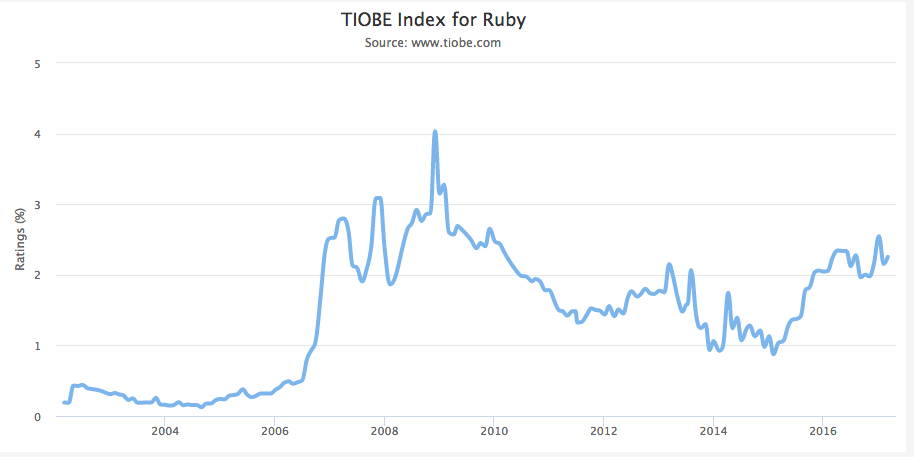
\includegraphics[width=1\linewidth]{pictures/ruby_tiobe}
  \caption{Histora popularności języka Ruby według rankingu Tiobe}
  \label{fig:ruby_tiobe}
\end{figure}


                                                                     




                                                                     




                                                                    





                                                                    





                                                                    





                                                                    





                                                                    





                                                                    






                                                                    








                                                                    








                                                                   









\begin{figure}[H]
  \centering
  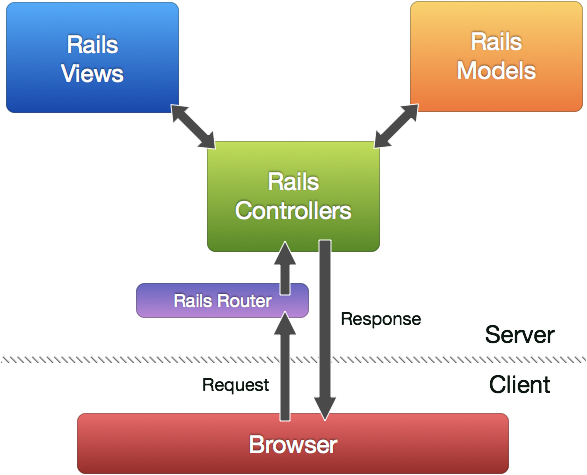
\includegraphics[width=1\linewidth]{pictures/rails_mvc}
  \caption{Architektura aplikacji w~Ruby on Rails, źródło: http://blog.ifuturz.com/ruby-on-rails/ruby-on-rails-mvc-learn-with-fun.html}
  \label{fig:rails_mvc}
\end{figure}
\newpage
Dwie główne zasady frameworku\cite{doc_rails}:


                                                                   









\begin{figure}[H]
  \centering
  \begin{forest}
    pic dir tree,
    where level=0{}{% folder icons by default; override using file for file icons
      directory,
    },
    [project\_root
      [app
        [controllers]
        [models]
        [views]
      ]
    ]
  \end{forest}
  \caption{Podstawowa struktura projektu Ruby on Rails}
  \label{fig:rails_structure}
\end{figure}


                                                                   









                                                                   











                                                                   











                                                                   











\begin{figure}[H]
  \centering
  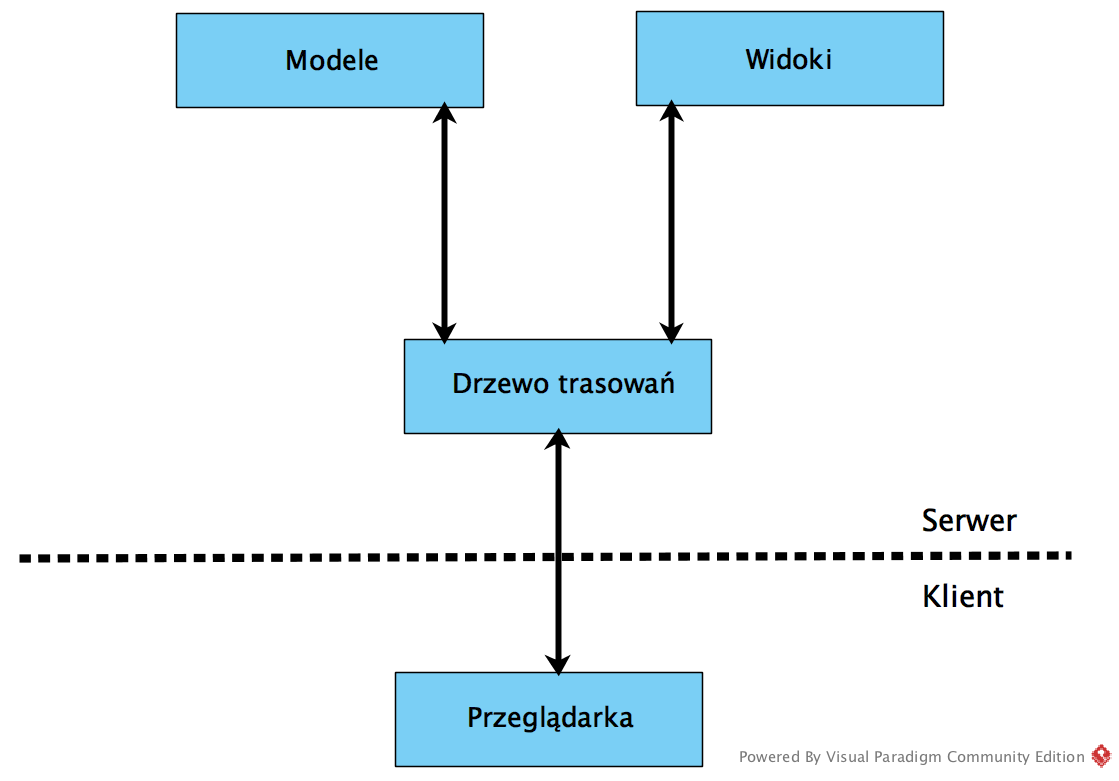
\includegraphics[width=1\linewidth]{pictures/roda_architecture}
  \caption{Architektura aplikacji w frameworku Roda}
  \label{fig:roda_architecture}
\end{figure}


\begin{figure}[H]
  \centering
  \begin{forest}
    pic dir tree,
    where level=0{}{% folder icons by default; override using file for file icons
      directory,
    },
    [project\_root
      [models]
      [routes]
      [views]
    ]
  \end{forest}   
  \caption{Struktura projektu Roda}
  \label{fig:roda_proj_structure}
\end{figure}


                                                                   











                                                                   











                                                                   











  \begin{figure}[H]
    \centering
    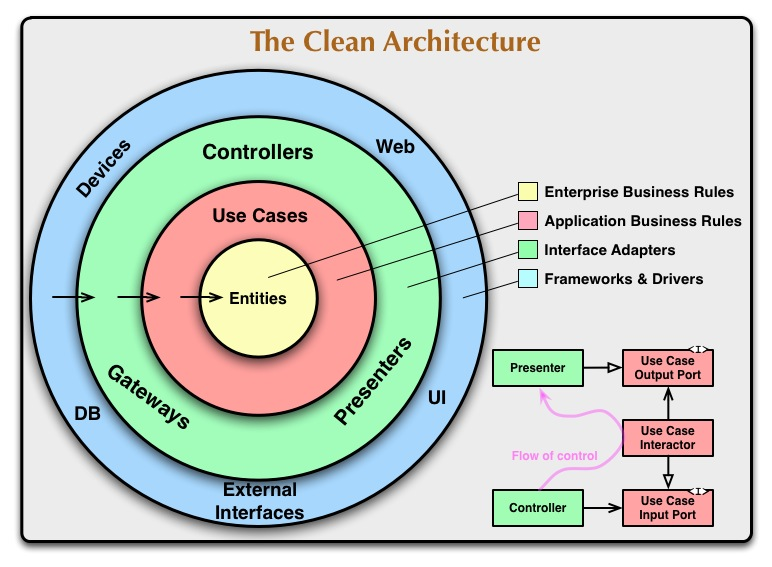
\includegraphics[width=1\linewidth]{pictures/clean_architecture}
    \caption{Schemat czystej architektury\cite{clean_architecture}}
    \label{fig:clean_architecture}
  \end{figure}


                                                                   











                                                                   












                                                                   












                                                                   












                                                                   












\begin{figure}[H]
  \centering
  \begin{forest}
    pic dir tree,
    where level=0{}{% folder icons by default; override using file for file icons
      directory,
    },
    [project\_root
      [apps
        [web
          [controllers]
          [templates]
          [views]
        ]
      ]
      [lib
        [main
          [entities]
          [repositories]
        ]
      ]
    ]
  \end{forest}
  \caption{Podstawowa struktura projektu Hanami}
  \label{fig:hanami_structure}
\end{figure}


                                                                   

















                                                                  


















                                                                  



















                                                                  



















                                                                  



















                                                                  



















                                                                  



















                                                                  



















                                                                  



















                                                                  



















                                                                  



















                                                                  



















                                                                  



















                                                                  



















                                                                  



















                                                                  



















                                                                  



















                                                                  



















                                                                  



















                                                                  



















                                                                  



















                                                                  



















                                                                  



















                                                                  



















                                                                  



















                                                                  



















                                                                  



















